\documentclass[12pt]{article}

%% preamble: Keep it clean; only include those you need
\usepackage{amsmath}
\usepackage[margin = 1in]{geometry}
\usepackage{graphicx}
\usepackage{booktabs}
\usepackage{natbib}
\usepackage{acronym}


%% for double spacing
\usepackage{setspace}

% for space filling
\usepackage{lipsum}
% highlighting hyper links
\usepackage[colorlinks=true, citecolor=blue]{hyperref}


%% meta data

\title{Stats Paper}
\author{Jesse DiMarzo\\
  Statistics Major, Mathematics Minor \\
  University of Connecticut
}

\begin{document}
\maketitle

\begin{abstract}

\begin{acronym}
    \acro{UFC}{Ultimate Fighting Championship}
\end{acronym}

As defined by the \ac{UFC}, the study aims to investigate the effects of repeated trauma to the head, which are apparent in the decline of motor skills, as seen in the declination of athletic performance.

\end{abstract}

\doublespacing

\section{Introduction}
\label{sec:intro}


The effects of repeated head trauma in sports are significant, affecting athletes' long-term health and performance

\lipsum[1]

Various sources have been used...
\citet{smith2020study} did something ... \lipsum[1]

A significant amount of research as been conducted by \citep[e.g.,][]{smith2020study}.
\lipsum[1]
A typical statistical analysis was performed by
\citet{smith2020analysis}. 


% roadmap
The rest of the paper is structured as follows.
Section~\ref{sec:data} presents the data.
Section~\ref{sec:meth} describes the methods used.
Section~\ref{sec:resu} reports the results.
Section~\ref{sec:disc} discusses the conclusion of the research.


\section{Data}
\label{sec:data}

This section provides a description of the data used to analyze the effects of 
repeated head trauma on motor skills, as seen in martial arts.

For example, consider the equation
\begin{equation}
  \label{eq:mc2}
  E = m c^2,
\end{equation}
which states that the energy $E$ of a particle in its rest frame as the product
of mass ($m$) with the speed of light squared ($c^2$).
\lipsum{1}

\section{Methods}
\label{sec:meth}

This section outlines the methodologies used to analyze the data on head trauma, using statistical models.

Suppose that the radius of a circle is $r$. Then its area is
\begin{equation}
  \label{eq:area}
  \pi r^2.
\end{equation}

Equation~\eqref{eq:area} is interesting. \lipsum[1]



\section{Results}
\label{sec:resu}

Table~\ref{tab:trauma_performance} summarizes some example the relationship between head trauma and motor performance decline in athletes.  \lipsum[1]

\lipsum[1]

\begin{table}[tbp]
  \caption{Trauma and Performance Data Summary.}
  \label{tab:trauma_performance}
\centering
\begin{tabular}{rrr}
  \toprule
Trauma Level & Motor Skill Score & Recovery Time \\ 
  \midrule
  1 & 85 & 1.5 \\ 
  2 & 78 & 2.0 \\ 
  3 & 72 & 2.5 \\ 
  4 & 65 & 3.0 \\ 
  5 & 60 & 3.5 \\ 
   \bottomrule
\end{tabular}
\end{table}

Figure~\ref{fig:performance_decline} shows a plot of motor skill score against trauma level... \lipsum[1]



\begin{figure}[tbp]
  \centering
  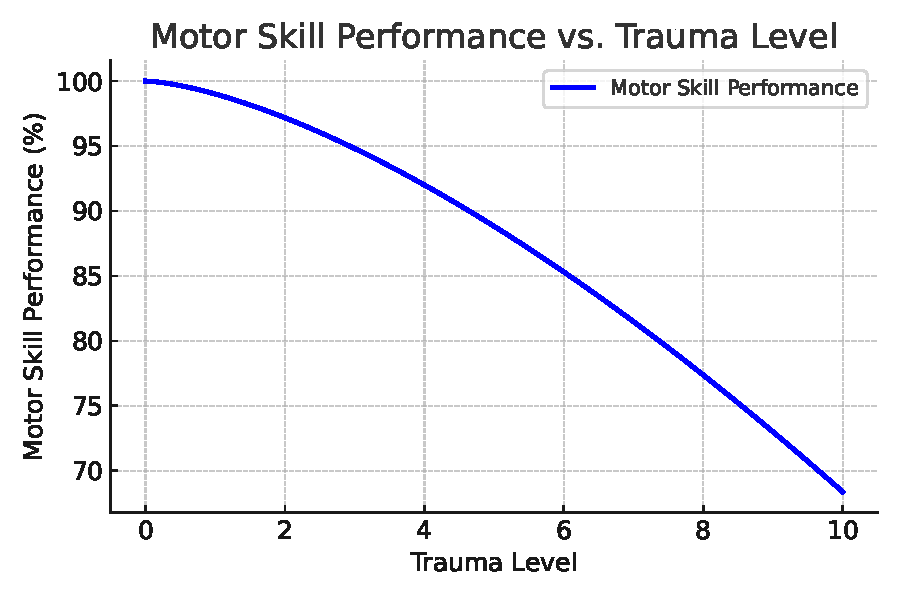
\includegraphics[width=\textwidth]{performance_decline.pdf}
  \caption{Motor skill score vs. trauma level.}
  \label{fig:performance_decline}
\end{figure}

\section{Discussion}
\label{sec:disc}

The main contribution of this study is to provide... \lipsum[1]

There are several limitations to this study. \lipsum [1]

\lipsum[1]
Further investigation is required to understand... \lipsum[1]

\bibliography{reference}
\bibliographystyle{mcap}

\end{document}